\documentclass[hyperref,a4paper,UTF8]{ctexart}

\usepackage[left=2.50cm, right=2.50cm, top=2.50cm, bottom=2.50cm]{geometry}

\usepackage[unicode=true,colorlinks,urlcolor=blue,linkcolor=blue,bookmarksnumbered=true]{hyperref}
\usepackage{latexsym,amssymb,amsmath,amsbsy,amsopn,amstext,amsthm,amsxtra,color,bm,calc,ifpdf}
\usepackage{graphicx}
\usepackage{enumerate}
\usepackage{fancyhdr}
\usepackage{listings}
\usepackage{multirow}
\usepackage{makeidx}
\usepackage{xcolor}
\usepackage{fontspec}
\usepackage{subfigure}
\usepackage{hyperref}
\usepackage{appendix}
\usepackage{pythonhighlight}
\usepackage{booktabs}
\usepackage{algorithm,algpseudocode}
\setmonofont{Consolas}

\pagestyle{fancy}
\fancyhead[L]{}
\fancyhead[C]{\kaishu 页眉 \qquad 冯超 \qquad 22210690089}
\fancyhead[R]{}

\title{\textbf{{标题}}}
\author{
  \kaishu\normalsize
  姓名\ \underline{冯超} \qquad
  项目\ \underline{DS\&BA} \qquad
  学号\ \underline{22210690089}
}
\date{} % 留空,不显示日期

\begin{document}

\maketitle

\tableofcontents

\section{标题}

\subsection{公式}

$$
    R_{it}^e =\alpha_i+\beta_i ^\prime \lambda_t+\varepsilon_{it},\quad t=1,2,\dots, T
$$

\subsection{算法}

\begin{algorithm}[H]
    \caption{坐标下降法}\label{坐标下降法}
    \hspace*{\algorithmicindent} \textbf{Input} 步长减小的参数$\alpha$($\alpha>0$), 最大迭代次数$K$, 迭代初始值$\boldsymbol{\beta}^0$\\
    \hspace*{\algorithmicindent} \textbf{Output} 迭代$K$次后得到的$\boldsymbol{\beta}$
    \begin{algorithmic}[1]
        \Function{coordinate\_descent}{$\alpha,K,\boldsymbol{\beta}^0$}
        \State $t_0 \leftarrow 1$, $\boldsymbol{\beta} \leftarrow \boldsymbol{\beta}^0$
        \For{$k\leftarrow 0$ to $(K-1)$}
        \State $t_k \leftarrow (k+1) ^{-\alpha}$
        \State $j = k \% \beta.shape$ \Comment{循环更新每个分量}
        \State $\boldsymbol{\beta}_{j} \leftarrow \boldsymbol{\beta}_{j}-t_k \nabla f_j(\boldsymbol{\beta})$
        \EndFor
        \State \textbf{return} $\boldsymbol{\beta}$
        \EndFunction
    \end{algorithmic}
\end{algorithm}

\subsection{代码}

\begin{python}
    print('Hello World')
\end{python}

\subsection{图片}

\subsubsection{单张图片}

\begin{figure}[H]
    \centering
    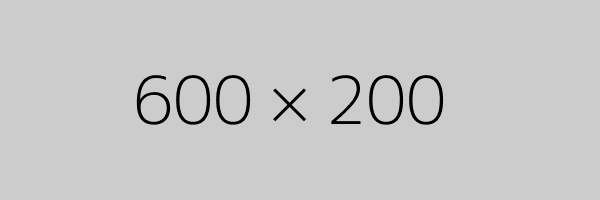
\includegraphics[width=0.5 \textwidth]{./image.png}
    \caption{图片标题}
\end{figure}

\subsubsection{多张图片并排}

\begin{figure}[H]
    \centering
    \begin{minipage}[t]{0.48\textwidth}
        \centering
        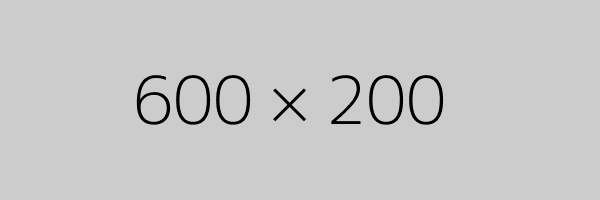
\includegraphics[width=1\textwidth]{./image.png}
        \caption{标题 1}\label{标题 1}
    \end{minipage}
    \begin{minipage}[t]{0.48\textwidth}
        \centering
        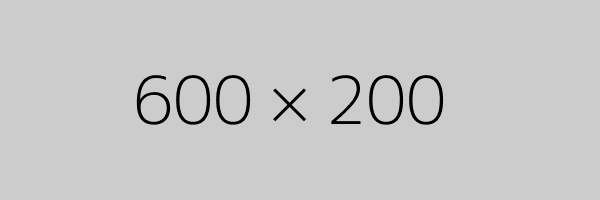
\includegraphics[width=1\textwidth]{./image.png}
        \caption{标题 2}\label{标题 2}
    \end{minipage}
\end{figure}

\subsection{列表}

\begin{itemize}
    \item
          文本
    \item
          文本
\end{itemize}

\begin{enumerate}
    \item
          文本
    \item
          文本
\end{enumerate}

\end{document}